\documentclass[svgnames]{beamer}

\usepackage{csspace-slides}

\title{Удивительная алгебра сравнения строк (часть 2)}

\author{\texorpdfstring{
    \Author{А. В. Тискин}{DPhil (Oxford),\ \ доцент МКН СПбГУ}
    \Author{Б. Золотов}{аспирант МКН СПбГУ}
}{}}


\begin{document}

\maketitle


\begin{frame}{\(\frac{3}{4}\)-local LCS}

\begin{center}
  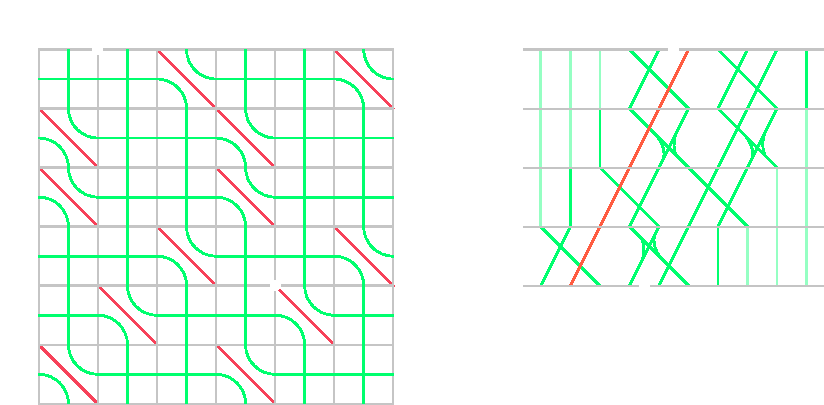
\includegraphics[width=9cm]{svg/34-local}
\end{center}

\end{frame}


\begin{frame}{Dynamic LCS}

\begin{center}
  
\includegraphics[width=4cm]{svg/dynamic}
\end{center}

\end{frame}


\begin{frame}{Грассмановы перестановки}

\begin{center}
  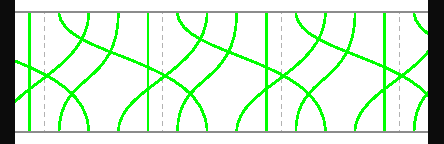
\includegraphics[width=6.4cm]{img-fg/tP}
  
  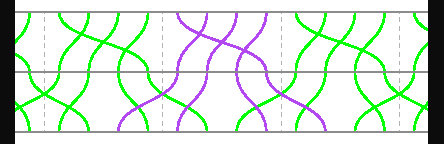
\includegraphics[width=6.4cm]{img-fg/tP-FG}

  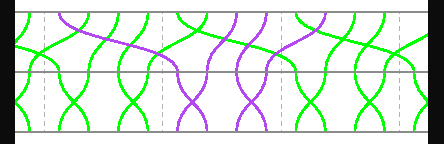
\includegraphics[width=6.4cm]{img-fg/tP-GF}
\end{center}

\end{frame}


\begin{frame}{Аффинное липкое умножение}

\begin{center}
  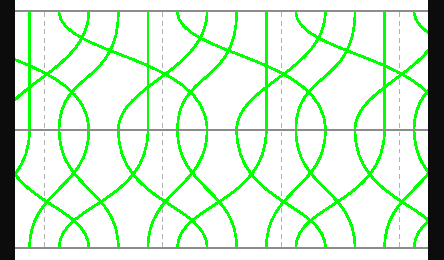
\includegraphics[width=4.5cm]{img-fg/PQ-base} \hspace{4mm}
  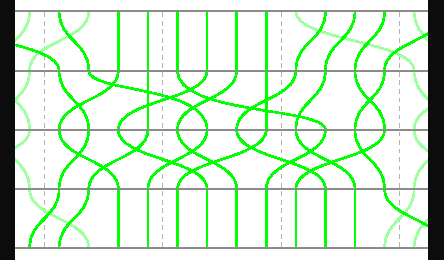
\includegraphics[width=4.5cm]{img-fg/PQ-GF3n} \vspace{2mm}

  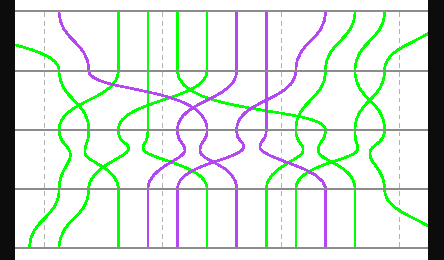
\includegraphics[width=4.5cm]{img-fg/PQ-GF3n-untg} \hspace{4mm}
  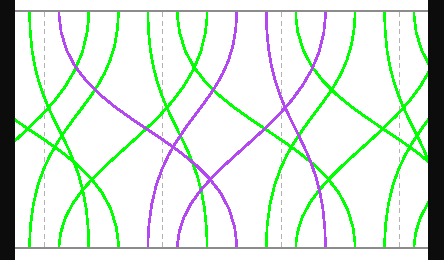
\includegraphics[width=4.5cm]{img-fg/PQ-GF3n-z}  
\end{center}

\end{frame}


\begin{frame}{Периодическая задача LCS}
\end{frame}


\end{document}
